\begin{figure} [h]
         \centering
         \caption{Analyse der Konditionszahlen gegen die Berechnungsergebnisse eines Messpunktes; Auffällig ist, dass die Lösungen für Referenzantenne 0 und 7 praktisch \textbf{keine} korrekte Lösung liefern. }
         \label{fig:CondNumberAnalyze}
%         
         \begin{subfigure}[t]{0.4\textwidth}
                 \centering
                 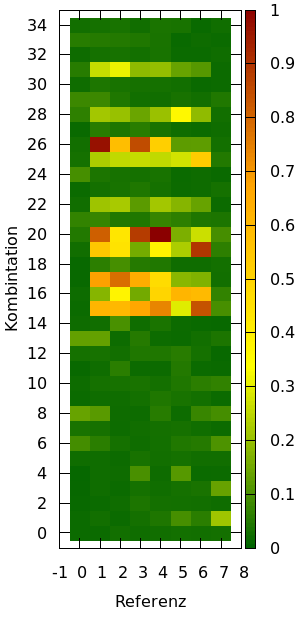
\includegraphics[width=\textwidth]{common/img/ConditionPlot_scaled.png}
                 \caption{Farbkodierte Matrix der Kondition aller möglichen Kombinationen (skaliert auf den höchsten vorkommenden Wert)\\
                 B=> grün~:=~gute -, rot=~schlechte Konditionierung}
                 \label{fig:ConditionMatrix}\textit{}
         \end{subfigure}
%         
\qquad
         \begin{subfigure}[t]{0.4\textwidth}
                 \centering
                 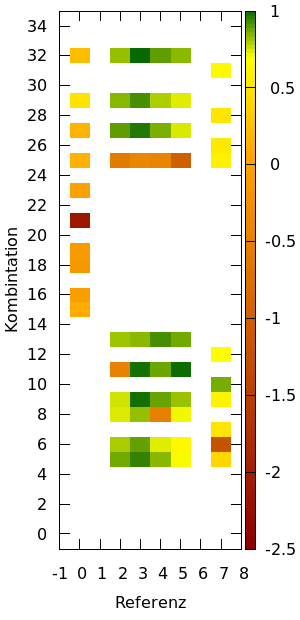
\includegraphics[width=\textwidth]{common/img/60_Results_scaled.png}
                 \caption{ Farbkodierte Ergebnisse der möglichen Kombinationen aus 6 von 8 Antennen; Die Position des Ergebnisses in der Matrix entspricht der in der Konditionsmatrix ddddddddd ddddddd dddddd dddddddddddddddddd.}
                 \label{fig:Results}
         \end{subfigure}
%
\end{figure}
